%#!pdfplatex
\documentclass{article}
\usepackage{graphicx}
\title{Fundamental Exercise on Computer and Information Engineering 1B \\ Ncurses Game}
\author{XL15613   Thiago Machado da Silva}
\date{\today}

\begin{document}
\maketitle

\section*{Output}
In Figure~\ref{fig:output} the game is shown, where a Game Over occurs. When I enlarge the screen this big, the game becomes too hard to win. \\

\begin{figure}[htbp]
  \makebox[\textwidth][c]{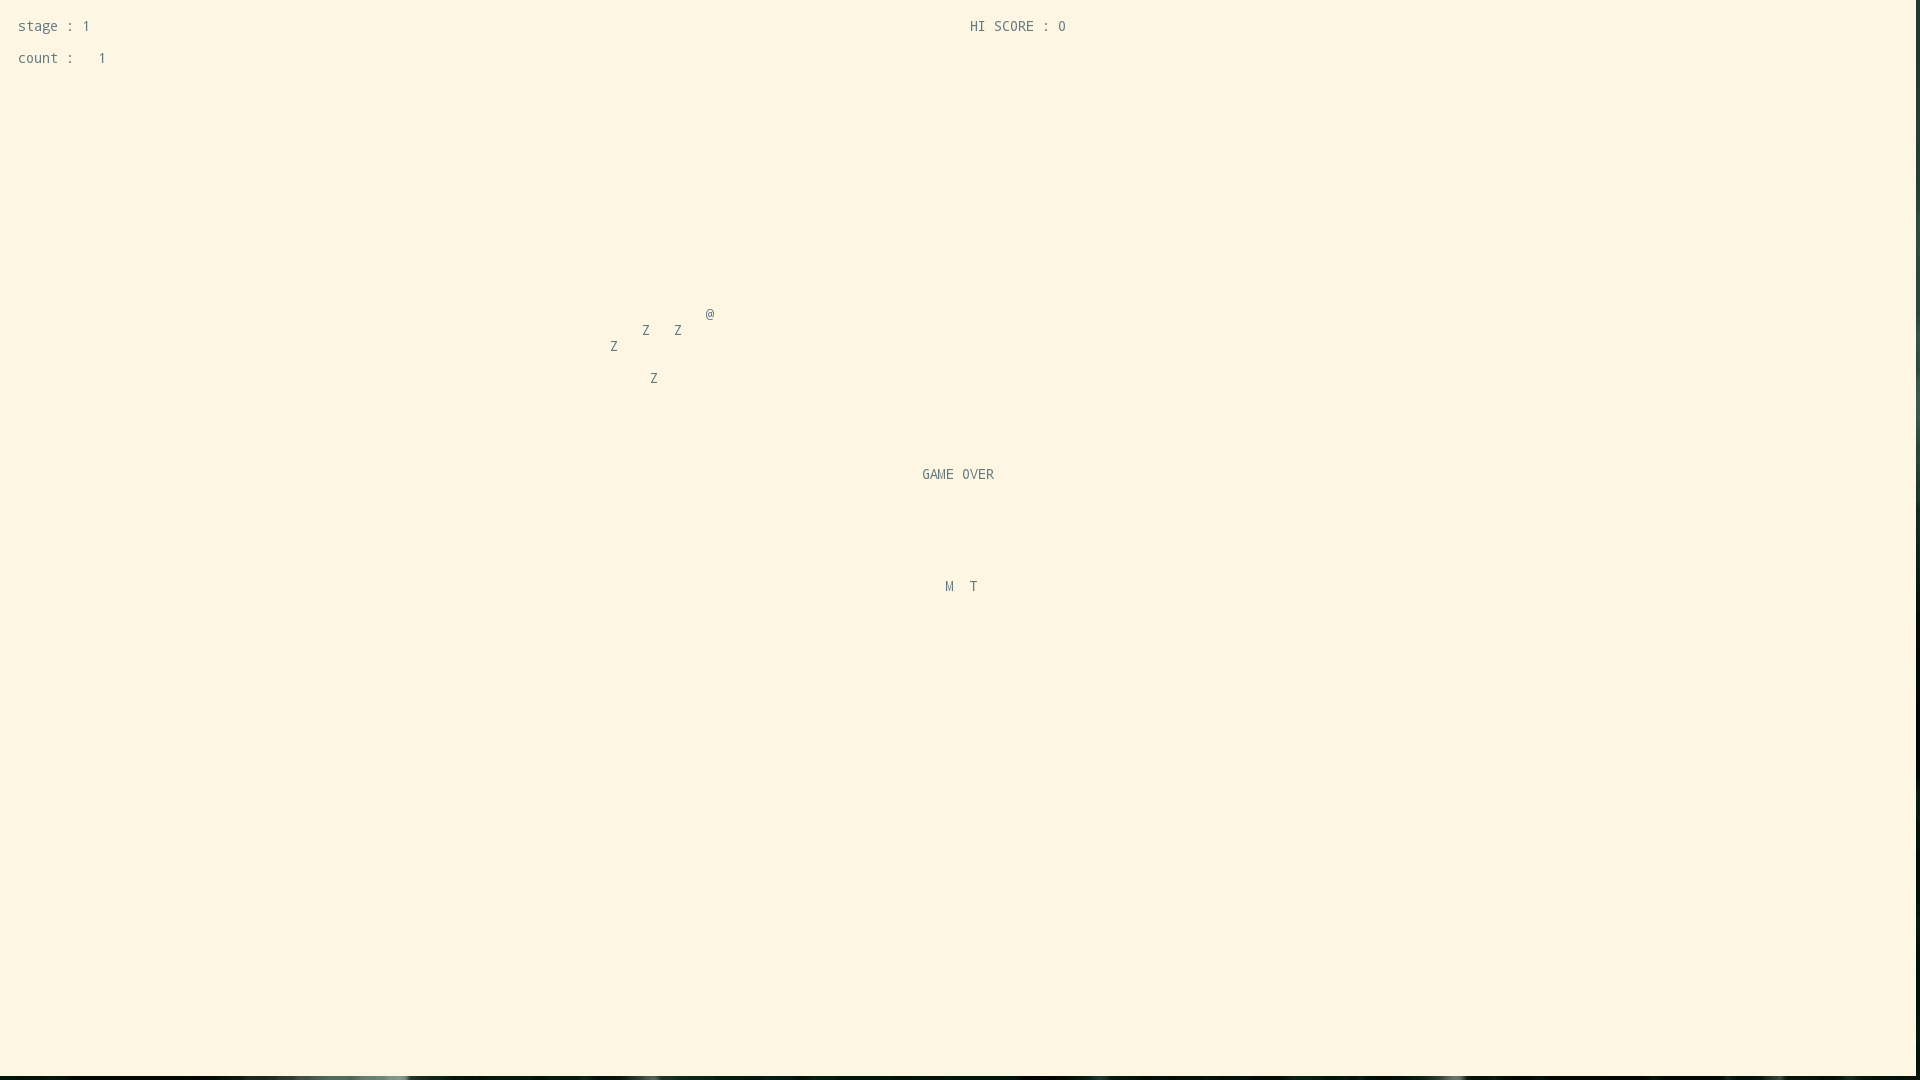
\includegraphics[width=1.78\textwidth]{./output.png}}%
  \centering
  \caption{Game execution.}
  \label{fig:output}
\end{figure}

\section*{Source codes}
Shown in Figure~\ref{fig:src1}.

\begin{figure}[h]
  \makebox[\textwidth][c]{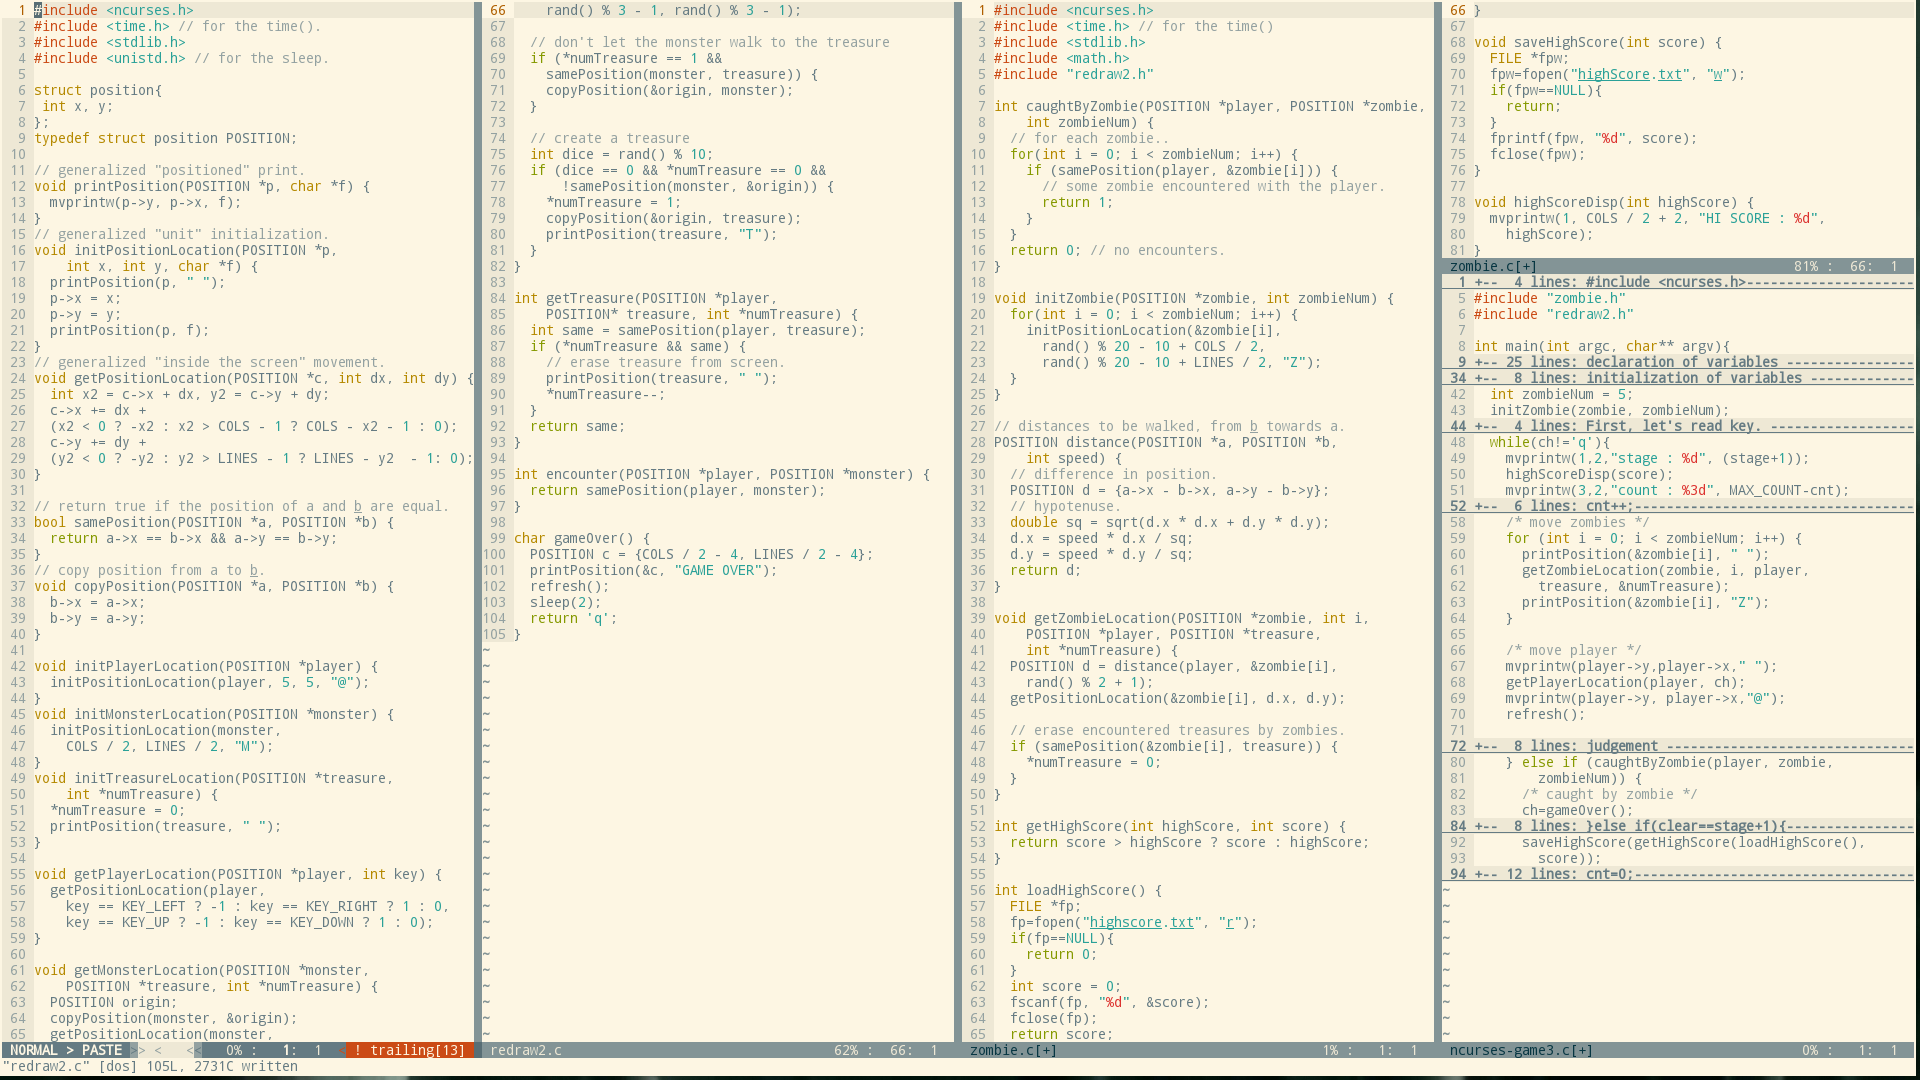
\includegraphics[width=1.78\textwidth]{./src1.png}}%
  \centering
  \caption{from left to right, top to bottom: {\tt redraw2.c} (until line 65), {\tt redraw2.c} (from line 66), {\tt zombie.c} (until line 65), {\tt zombie.c} (from line 66) and {\tt ncurses-game3.c} (only the highlights).}
  \label{fig:src1}
\end{figure}

\end{document}
